\subsection{Rayleigh-Taylor Instability}

This problem is based on the evolution of two layers of fluids initially at rest in a gravity field. The density of the upper most fluid is larger than the one placed underneath. Due to a little disturbance in the contact surface the more dense fluid moves down and the less dense fluid does the opposite. During the evolution of the problem, a mixture is created, which is lately segregated. The final state reaches an stable equilibrium with the more dense fluid at the bottom layer and the less dense fluid at the top layer. The growth and evolution of the instability has been investigated among others by Tryggvason\cite{Tryggvason88} for inviscid incompressible flows, and by Guermond \& Quartapelle\cite{Guermond00} for viscous flows.

The starting point is the problem documented by Guermond\cite{Guermond00}. The computational domain is $[-d/2,d/2]\times[-2d,2d]$ and the initial position of the perturbed interface is $\eta(x) = 0.1d \cos(2\pi x/d)$. The density ratio is $3$, which corresponds to an Atwood
number of $0.5$ according to Tryggvason's definition $At = (\rho_{max}-\rho_{min})/(\rho_{max}+\rho_{min})$. Other physical parameters are selected to obtain a Reynolds number $Re=\rho_{min}d^{\frac{3}{2}}g^{\frac{1}{2}}/\mu=1000$. The computational domain is discretized into $80000$ structured triangles ($\Delta x=0.01$) setting slip boundary conditions on each wall. The time step selected is $\Delta t=0.01[s]$, which allows for $CFL_{max} \approx 8$. Between five and eight particles per element are used and two pressure iterations are required.

To compare solutions with reference results, the time is made dimensionless by using $\widetilde{t} = t\sqrt{g\ At}$. Results on the vertical position of the tip of the falling and rising fluid (spike and bubble, respectively) are shown in Figure \ref{fg:rayleigh-rf}. It can be observed that current solution is in good agreement with the reference results.

\begin{figure}[H]
  \begin{center}
      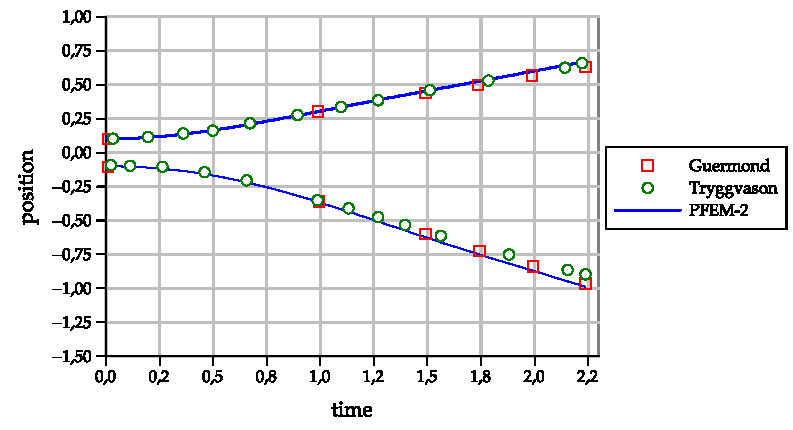
\includegraphics[width=\columnwidth]{images/rayleigh_1.pdf}
  \end{center}
  \caption{\label{fg:rayleigh-rf} Position of rising and falling bubbles versus time. Case with $Re=1000$.}
\end{figure}

On the other hand, the evolution of the instability is shown in Figure \ref{fg:rayleigh-screenshots} at dimensionless times $\widetilde{t}=0, 1, 1.5, 2$. Around $\widetilde{t}=1.5$ the heavy fluid begins to roll up into two counter-rotating vortices. Later, around $\widetilde{t} = 2$, these two vortices become unstable and a pair of secondary vortices appear at the tails of the roll-ups. These shapes of the fluid interface obtained with PFEM-2 are similar to the ones shown as reference results, see \cite{Guermond00}.


\begin{figure}[htbp]
  \begin{center}
      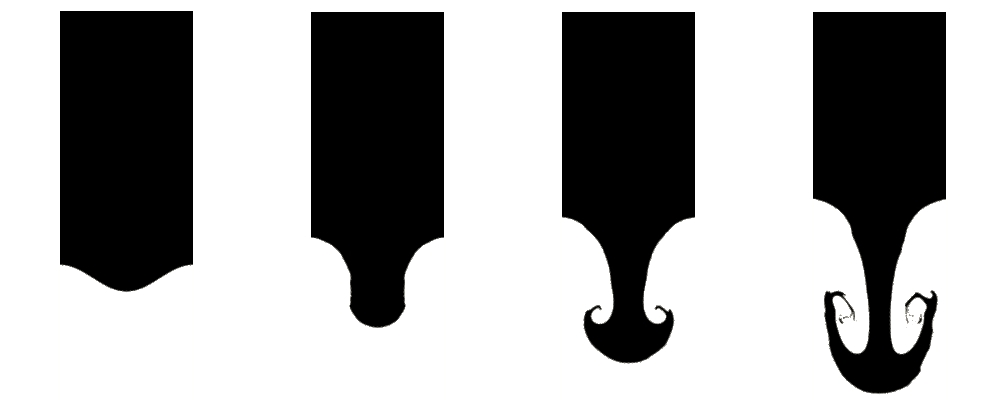
\includegraphics[width=\columnwidth]{images/rayleigh_2_better.jpg}
  \end{center}
  \caption{\label{fg:rayleigh-screenshots} Rayleigh-Taylor instability evolution. Case with $Re=1000$. From left to right $\widetilde{t} =0.0$, $1.0$, $1.5$, $2.0$.}
\end{figure}

\subsubsection{Extending the time step}

In order to emphasize the capability of the method to manage large time-steps, the current case is also simulated with a large range of $\Delta t$ using the in-house implementation of PFEM and comparing with results obtained by the widely known \OF suite. The problem setup and domain discretization is the same as presented above and the PFEM settings are not modified.

In the case of \OF, the solver \texttt{interFoam} is chosen, which implements a Volume of Fluid (VoF) algorithm for multiphase flow\cite{Berberovic09}\cite{Marquez2014}. It includes the multi-dimensional limiter for explicit solution (MULES) as a method of guaranteeing boundedness of scalar fields, in particular phase/mass-fractions (more information about MULES can be found in \cite{Marquez13}). Since \OF version 2.3, a new semi-implicit variant of MULES has been introduced which combines operator splitting with application of the MULES limiter to an explicit correction rather than to the complete flux. This approach would maintain boundedness and stability at an arbitrarily large Courant number. In the next simulation, the following recommended simulation schemes have been used: \texttt{CrankNicolson} (second order, implicit) time integration, \texttt{Gauss linear} (second order, Gaussian integration with linear interpolation) discretization for the gradient, divergence and Laplacian operators (\texttt{
corrected} with two \texttt{nNonOrthogonalCorrectors} due to the triangular mesh, for the later ). Relevant VoF settings are: \texttt{nAlphaSubCycles} is set in order to keep the CFL of the sub-cycling around $0.5$, \texttt{cAlpha}$=0.25$ to give more stability through relaxing on some level the strong sharpness imposition, and \texttt{MULESCorr} is enabled to calculate the limiter in a semi-implicit way.

Figure \ref{fg:rayleigh-comparison-dts} presents the comparison of the solutions with PFEM and \OF at a particular time ($\widehat{t}=2.25$) using several fixed time-steps (with the largest time-step reaching a $CFL_{max}=15$). From captures, it can be shown that PFEM keeps approximately the same solution with each time-step, but interFoam can not solve with any accuracy using $\Delta t>0.001$ because the evolution of the mushroom-like interface differs form the reference results and this divergence is increased with larger time-steps. Moreover, simulations with interFoam diverge when $CFL_{mean}>0.5$ is reached (this happens at different times, depending on the selected time-step).

\begin{figure}[htbp]
  \begin{center}

      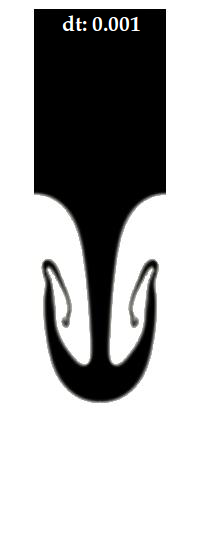
\includegraphics[width=.24\columnwidth]{images/rayleigh_foam_dts_A.png}
      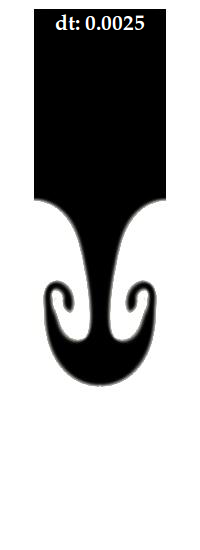
\includegraphics[width=.24\columnwidth]{images/rayleigh_foam_dts_B.png}
      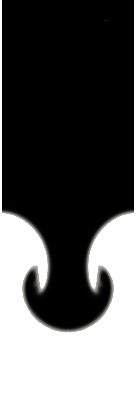
\includegraphics[width=.24\columnwidth]{images/rayleigh_foam_dts_C.jpg}
      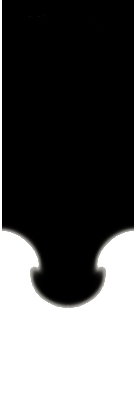
\includegraphics[width=.24\columnwidth]{images/rayleigh_foam_dts_D.jpg}

      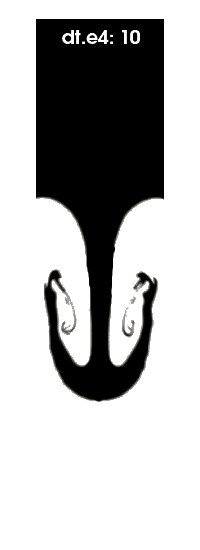
\includegraphics[width=.24\columnwidth]{images/rayleigh_pfem_dts_A.jpg}
      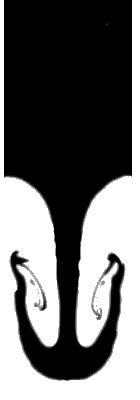
\includegraphics[width=.24\columnwidth]{images/rayleigh_pfem_dts_B.jpg}
      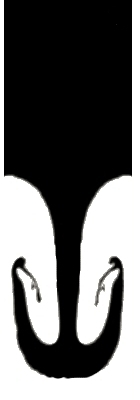
\includegraphics[width=.24\columnwidth]{images/rayleigh_pfem_dts_C.jpg}
      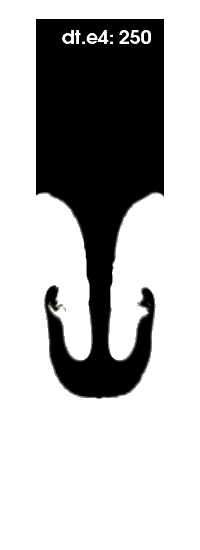
\includegraphics[width=.24\columnwidth]{images/rayleigh_pfem_dts_D.jpg}

  \end{center}
  \caption{\label{fg:rayleigh-comparison-dts} Rayleigh-Taylor instability capture for $\widetilde{t}=2.25$. Bottom: PFEM simulations, top: VoF+MULES simulation (InterFoam solver - OpenFoam suite). From left to right $\Delta t =0.001[s]$, $0.0025[s]$, $0.01[s]$, $0.025[s]$.}
\end{figure}

Another relevant feature to take into account when comparing both algorithms is that similar CPU times are required to solve a time-step.
Table \ref{tb:times-rt} summarizes the CPU Times required to complete $1[s]$ of real time in the current case. Results show that, using the same time-step, both solvers have similar performance, being \OF faster. However, due to the capability of time-step enlargement with PFEM, shorter CPU times are achieved with similar accuracy.

{\small
\begin{longtable}{||c|c||c||}
    \hline
    Solver & $\Delta t$ & CPU Time\\
      \hline
      \hline
      \OF & 0.001 & 1121[s]\\
      PFEM & 0.0025 & 1011[s]\\
      PFEM & 0.01 & 288[s]\\
      PFEM & 0.025 & 123[s]\\
      \hline
      \hline
    \caption{\label{tb:times-rt} Total computing times to simulate $1[s]$ of real time of the Rayleigh-Taylor instability 2d. Running on an Intel i5-3230M CPU @ 2.60GHz with 8Gb of RAM and one processor.}
\end{longtable}
}

\subsubsection{Three-dimensional simulation}

In this section, the extension of the two dimensional problem to three dimensions is presented. The third dimension is generated as a surface of revolution from the previous 2d geometry, conforming a cylindrical volume in 3d of radius $R=0.5$. This allows the same problem configuration to be kept, this is, a slip boundary condition on the wall, $At=0.5$, and an initial perturbation of the surface $\eta(r) = 0.1d \cos(2\pi r/d)$, with $0<r<R$.

The computational domain is discretized with a mesh size of $\Delta x=0.03[m]$ conforming a non-structured mesh with around $1.2$ millon tetrahedral elements. An average of eight millon particles are used during the simulation that move across the light-phase and heavy-phase domains. Simulation was carried out with a $\Delta t=0.025$ which peaks to $CFL_{max}=15$. Figure \ref{fg:rayleigh-3d} shows the evolution of the heavy-phase. It must be noticed that the simulation is extended until reaching the stable condition with the heavy-phase at the bottom and at rest, which is approximately $30[s]$ of simulation time. To complete the entire simulation, the implementation requires around three hours of CPU running time on an AMD Opteron 6376 @ 2.3GHz with a 64Gb RAM using 16 processors.

As an additional result, it is important to underline that, during the simulation, the global mass conservation has been verified.

 However, the spirit of this section is to show the stability of the 3D simulation with a realistic progress. A way to prove the validity of the solution is that, during the simulation, the initial mass quantity is preserved. A more detailed analysis about the accuracy of 3d simulations will be presented in Section \ref{sec:ETSIN-3d}.

\begin{figure}[htbp]
  \begin{center}
    \subfloat[]{
	  \label{fg:RT-3d-a}
	  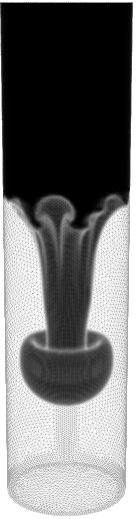
\includegraphics[width=.18\columnwidth]{images/RT_3d/RT3d_a.jpg}
    }
    \subfloat[]{
	  \label{fg:RT-3d-b}
	  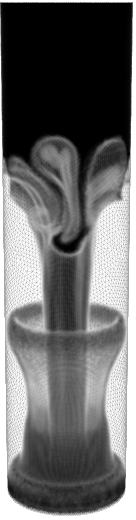
\includegraphics[width=.18\columnwidth]{images/RT_3d/RT3d_b.jpg}
    }
    \subfloat[]{
	  \label{fg:RT-3d-c}
	  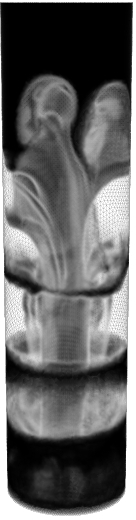
\includegraphics[width=.18\columnwidth]{images/RT_3d/RT3d_c.jpg}
    }
%     \subfloat[]{
% 	  \label{fg:RT-3d-d}
% 	  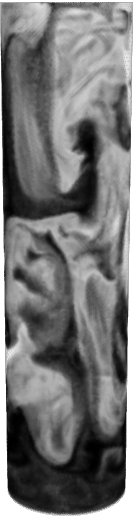
\includegraphics[width=.15\columnwidth]{images/RT_3d/RT3d_d.jpg}
%     }
    \subfloat[]{
	  \label{fg:RT-3d-e}
	  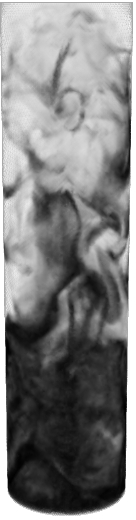
\includegraphics[width=.18\columnwidth]{images/RT_3d/RT3d_e.jpg}
    }
    \subfloat[]{
	  \label{fg:RT-3d-g}
	  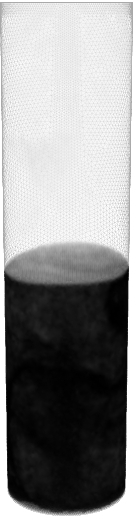
\includegraphics[width=.18\columnwidth]{images/RT_3d/RT3d_g.jpg}
    }
  \end{center}
  \caption{\label{fg:rayleigh-3d} Snapshots of the heavy-phase in the Rayleigh-Taylor instability solved in three-dimensions with PFEM-2. %From left to right $\widetilde{t} =2[s]$, $3.3[s]$, $4.4[s]$, $6.6[s]$, $8,8[s]$, and $27.5[s]$.}
  From left to right $\widetilde{t} =2[s]$, $3.3[s]$, $4.4[s]$, $8,8[s]$, and $27.5[s]$.}
\end{figure}

\afterpage{\clearpage}
